\subsection{Component}
\label{sec:Component}

The \sbol{Component} class represents the structural and/or functional entities of a biological design. The primary usage of this class is to represent entities with designed sequences, such as DNA, RNA, and proteins, but it can also be used to represent any other entity that is part of a design, such as simple chemicals, molecular complexes, strains, samples, light, and abstract functional groupings of other entities.

As shown in \ref{uml:component}, the \sbol{Component} class describes a design entity using the following properties: \sbolmult{type:CD}{type}, \sbolmult{role:CD}{role}, \sbol{hasSequence}, \sbol{hasFeature}, \sbol{hasConstraint}, \sbol{hasInteraction}, and \sbol{hasModel}.  The \sbol{hasSequence}, \sbol{hasFeature}, and \sbol{hasConstraint} properties are used to represent structural relationships, while the \sbol{hasInteraction} and \sbol{hasModel} are used to represent functional relationships.

\begin{figure}[ht]
\begin{center}
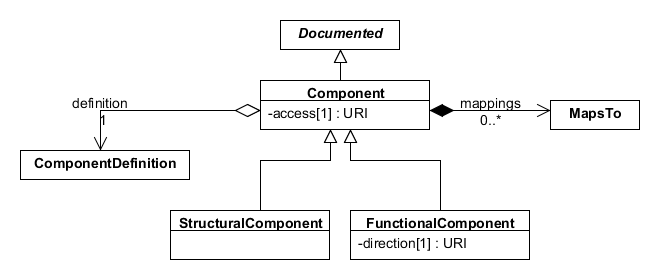
\includegraphics[width=0.95\textwidth]{uml/component}
\caption[]{Diagram of the \sbol{Component} class and its associated properties.}
\label{uml:component}
\end{center}
\end{figure} 

\subparagraph{The \sbolheading{type} property}
\label{sec:type:CD}

A \sbol{Component} is REQUIRED to have one or more \sbolmult{type:CD}{type} properties, each of type \sbol{URI} specifying the category of biochemical or physical entity (for example DNA, protein, or simple chemical) that a \sbol{Component} object abstracts
for the purpose of engineering design. For DNA or RNA entities, additional \sbolmult{type:CD}{type} properties are used to describe nucleic acid topology (circular / linear) and strandedness (double- or single-stranded).

The \sbolmult{type:CD}{type} properties of every \sbol{Component} MUST include one or more \sbol{URI}s that MUST identify terms from appropriate ontologies, such as the physical entity representation branch of the Systems Biology Ontology~\cite{SBO} or the ontology of Chemical Entities of Biological Interest (ChEBI)~\cite{chebi}.  \ref{tbl:component_types} provides a partial list of possible ontology terms for the \sbolmult{type:CD}{type} property and their \sbol{URI}s.  In order to maximize the compatibility of designs, the \sbolmult{type:CD}{type} property of a \sbol{Component} SHOULD contain a \sbol{URI} from the physical entity representation branch of the Systems Biology Ontology~\cite{SBO}, and any \sbol{Component} that can be well-described by one of the terms in \ref{tbl:component_types} MUST use the \sbol{URI} for that term as one of its \sbolmult{type:CD}{type}.
Finally, if the \sbolmult{type:CD}{type} property contains multiple \sbol{URI}s, then they MUST identify non-conflicting terms (otherwise, it might not be clear how to interpret them). For example, the SBO terms provided by \ref{tbl:component_types} would conflict because they specify classes of biochemical entities with different molecular structures.

\begin{table}[ht]
  \begin{edtable}{tabular}{ll}
    \toprule
    \textbf{Component Type} & \textbf{URI for SBO Term} \\
    \midrule
    DNA (Deoxyribonucleic acid)  & \url{https://identifiers.org/SBO:0000251}\\
    RNA (Ribonucleic acid) & \url{https://identifiers.org/SBO:0000250}\\
    Protein (Polypeptide chain)  & \url{https://identifiers.org/SBO:0000252}\\
    Simple Chemical  & \url{https://identifiers.org/SBO:0000247}\\
    Non-covalent complex  & \url{https://identifiers.org/SBO:0000253}\\
    Functional Entity  & \url{https://identifiers.org/SBO:0000241}\\
    \bottomrule
  \end{edtable}
  \caption{Partial list of the most common SBO terms to specify the molecule type using the \sbolmult{type:CD}{type} property of a \sbol{Component}.  Systems composed of multiple molecules composed together to perform a function should use the functional entity type.}
 \label{tbl:component_types}
\end{table}

\emph{Nucleic Acid Topology types}\\
Any \sbol{Component} classified as DNA (see \ref{tbl:component_types}) is RECOMMENDED to encode circular/linear topology information in an additional type field. This (topology) type field SHOULD specify a URI from the Topology Attribute branch of the SO
(this is currently just `linear' or `circular' as given in \ref{tbl:component_topology}). Topology information SHOULD be specified for DNA \sbol{Component} records with a fully specified sequence, except in three scenarios: if the DNA record does not have sequence information, or if the DNA record has incomplete sequence information, or if topology is genuinely unknown. For any \sbol{Component} classified as RNA (see \ref{tbl:component_types}), a topology type field is OPTIONAL. The default
assumption in this case is linear topology.  In any case, no more than one topology should be specified.

Any \sbol{Component} classified as DNA or RNA MAY also have strand
information encoded in an additional (third) type field using a URI from the Strand Attribute branch of the SO (currently there are only two possible terms for single or double-stranded nucleic
acids given in \ref{tbl:component_topology}). In absence of this field, the
default strand information assumed for DNA is `double-stranded' and for RNA is
`single-stranded'. 

Any other type of \sbol{Component} record (protein, simple chemical, etc) SHOULD NOT
have any type field pointing to SO terms from the topology or strand attribute branches of SO.

Note that a \emph{circular} topology instructs software to interpret the
beginning / end position of a given sequence (be it DNA or RNA) as arbitrary so
that sequence features may be mapped or identified across this junction. \emph{Double stranded} instructs software to apply sequence searches to both strands (i.e. sequence and reverse complement of sequence).

\begin{table}[ht]
  \begin{edtable}{tabular}{ll}
    \toprule
    \textbf{Nucleic Acid Topology} & \textbf{URI for Nucleic Acid Topology
      Term in SO} \\
    \midrule
    linear  & \url{http://identifiers.org/so/SO:0000987}\\
    circular  & \url{http://identifiers.org/so/SO:0000988}\\
    single-stranded & \url{http://identifiers.org/so/SO:0000984}\\
    double-stranded & \url{http://identifiers.org/so/SO:0000985}\\
    \bottomrule
  \end{edtable}
  \caption{Sequence Ontology terms to encode DNA or RNA topology information in the \sbolmult{types:CD}{types} properties of a \sbol{Component}.}
 \label{tbl:component_topology}
\end{table}

\subparagraph{The \sbolheading{role} property}
\label{sec:role:CD}

A \sbol{Component} MAY have one or more \sbolmult{role:CD}{role} properties, each of type \sbol{URI} that MUST identify terms from ontologies that are consistent with the \sbolmult{type:CD}{type} property of the \sbol{Component}.  For example, the \sbolmult{role:CD}{role} property of a DNA or RNA \sbol{Component} could contain URIs identifying terms from SO. As a best practice, a DNA or RNA \sbol{Component} SHOULD contain exactly one \sbol{URI} that refers to a term from the sequence feature branch of the SO.
Similarly, the role properties of a protein and simple chemical \sbol{Component} SHOULD respectively contain \sbol{URI}s identifying terms from the \texttt{MolecularFunction} branch (\texttt{GO:0003674}) of the Gene Ontology (GO) and the \texttt{role} branch (\texttt{CHEBI:50906}) of the CHEBI ontology.
\ref{tbl:component_roles} contains a partial list of possible ontology terms for the \sbolmult{role:CD}{role} properties and their \sbol{URI}s. These terms are organized by the type of \sbol{Component} to which they SHOULD apply (see \ref{tbl:component_types}). Any \sbol{Component} that can be well-described by one of the terms in \ref{tbl:component_roles} MUST use the \sbol{URI} for that term as one of its \sbolmult{role:CD}{role}.

These \sbol{URI}s might identify descriptive biological roles, such as ``metabolic pathway'' and ``signaling cascade,'' but they can also identify identify ``logical'' roles, such as ``inverter'' or ``AND gate'', or other abstract roles for describing the function of design. Interpretation of the meaning of such roles currently depends on the software tools that read and write them.

\begin{table}[ht]
  \begin{edtable}{tabular}{lll}
    \toprule
    \textbf{Component Role} & \textbf{URI for Ontology Term} & \textbf{Component Type} \\
    \midrule
   Promoter & \url{http://identifiers.org/so/SO:0000167} & DNA \\
   RBS & \url{http://identifiers.org/so/SO:0000139} & DNA \\
      CDS & \url{http://identifiers.org/so/SO:0000316} & DNA \\
      Terminator & \url{http://identifiers.org/so/SO:0000141} & DNA \\
      Gene & \url{http://identifiers.org/so/SO:0000704} & DNA \\
      Operator & \url{http://identifiers.org/so/SO:0000057} & DNA \\
      Engineered Gene & \url{http://identifiers.org/so/SO:0000280} & DNA \\
      mRNA & \url{http://identifiers.org/so/SO:0000234} & RNA \\
      Effector & \url{http://identifiers.org/chebi/CHEBI:35224} & Small Molecule \\
      Transcription Factor & \url{http://identifiers.org/go/GO:0003700} & Protein\\
    \bottomrule
  \end{edtable}
  \caption{Partial list of ontology terms to specify the \sbolmult{role:CD}{role} property of a \sbol{Component}, organized by the type of \sbol{Component} to which they are intended to apply (see \ref{tbl:component_types}).}
  \label{tbl:component_roles}
\end{table}

\subsubsection*{The \sbolheading{hasSequence} property}
\label{sec:hasSequence}
A \sbol{Component} MAY have one or more \sbol{hasSequence} properties, each of type \sbol{URI} that MUST reference a \sbol{Sequence} object (see \ref{sec:Sequence}).  These objects define the primary structure of the \sbol{Component}.

If a \sbol{Feature} of a \sbol{Component} refers to a \sbol{Location}, and this \sbol{Location} refers to a \sbol{Sequence}, then the \sbol{Component} MUST also include a \sbol{hasSequence} property that refers to this \sbol{Sequence}.

Many \sbol{Component} objects will have exactly one \sbol{hasSequence} property that refers to a \sbol{Sequence} object.  In this case, if its has a \sbolmult{type:CD}{type} from \ref{tbl:componentdefinition_types} and there is an \sbol{encoding} that is cross-listed with this term in \ref{tbl:sequence_encodings}, then the \sbol{Sequence} objects MUST have this encoding.
This \sbol{Sequence} is implicitly the entire sequence for this \sbol{Component} (In other words, it is equivalent to a \sbol{SequenceFeature} with an \sbol{EntireSequence} \sbol{Location} that refers to this \sbol{Sequence}).

\subparagraph{The \sbolheading{hasFeature} property}
\label{sec:hasFeature}

A \sbol{Component} MAY have one or more \sbol{hasFeature} properties, each of type \sbol{URI} that MUST reference a \sbol{Feature} object (see \ref{sec:Feature}). The set of relations between \sbol{Feature} and \sbol{Component} objects MUST be strictly acyclic.

While the \sbol{Component} class is analogous to a blueprint or specification sheet for a biological part or a system of interacting biological elements, the \sbol{Feature} class represents, among other things, the specific occurrence of a part or subsystem within a design.  For example, this mechanism allows a biological design to include multiple instances of a particular part (defined by reference to the same \sbol{Component}). For example, the \sbol{Component} of a polycistronic gene could contain two \sbol{SubComponent} objects that refer to the same \sbol{Component} of a CDS.  As another example, consider the \sbol{Component} for a network of two-input repressor devices in which the particular repressors have not been chosen yet. This \sbol{Component} could contain multiple \sbol{SubComponent} objects that refer to the same \sbol{Component} of an abstract two-input repressor device.

The \sbol{hasFeature} properties of \sbol{Component} objects can be used to construct a hierarchy of \sbol{SubComponent} and \sbol{Component} objects.  If a \sbol{Component} in such a hierarchy refers to a \sbol{Location} object, and there exists a \sbol{Component} object lower in the hierarchy that refers to a \sbol{Location} object that refers to the same \sbol{Sequence} with the same \sbol{encoding}, then the \sbol{elements} properties of these \sbol{Sequence} objects SHOULD be consistent with each other, such that well-defined mappings exist from the ``lower level'' \sbol{elements} to the ``higher level'' \sbol{elements} in accordance with their shared \sbol{encoding} properties. This mapping is also subject to any restrictions on the positions of the \sbol{Feature} objects in the hierarchy that are imposed by the \sbol{SubComponent}, \sbol{SequenceFeature}, or \sbol{SequenceConstraint} objects contained by the \sbol{Component} objects in the hierarchy.

A DNA \sbol{Component}, for example, could refer to a \sbol{Sequence} with an \external{IUPAC DNA} \sbol{encoding} and an \sbol{elements} \external{String} of ``{\tt gattaca}.'' In turn, this \sbol{Component} could contain a \sbol{SubComponent} that refers to a ``lower level''  \sbol{Component} that also refers to a \sbol{Sequence} with an \external{IUPAC DNA} \sbol{encoding}. Consequently, a consistent \sbol{elements} \external{String} of this ``lower level'' \sbol{Sequence} could be ``{\tt gatta},'' or perhaps ``{\tt tgta}'' if the \sbol{SubComponent} is positioned by a \sbol{Location} with an \sbol{orientation} of ``reverse complement'' (see \ref{sec:Location}).

\subparagraph{The \sbolheading{hasConstraint} property}
\label{sec:hasConstraint}

A \sbol{Component} MAY have one or more \sbol{hasConstraint} properties, each of type \sbol{URI} that MUST reference a \sbol{Constraint} object (see \ref{sec:Constraint}).  These objects describe, among other things, any restrictions on the relative, sequence-based positions and/or orientations of the \sbol{Feature} objects contained by the \sbol{Component}.
For example, the \sbol{Component} of a gene might specify that the position of its promoter \sbol{SubComponent} precedes that of its CDS \sbol{SubComponent}. This is particularly useful when a \sbol{Component} lacks a \sbol{Sequence} and therefore cannot specify the precise, sequence-based positions of its \sbol{SubComponent} objects using \sbol{Location} objects.

\subparagraph{The \sbolheading{hasInteraction} property}\label{sec:hasInteraction}

A \sbol{Component} MAY have one or more \sbol{hasInteraction} properties, each of type \sbol{URI} that MUST reference an \sbol{Interaction} object (see \ref{sec:Interaction}).  

The \sbol{Interaction} class provides an abstract, machine-readable representation of entity behavior within a \sbol{Component} (whereas a more detailed model of the system might not be suited to machine reasoning, depending on its implementation).
Each \sbol{Interaction} contains \sbol{Participation} objects that indicate the roles of the \sbol{Feature} objects involved in the \sbol{Interaction}.

\subparagraph{The \sbolheading{hasModel} property}\label{sec:hasModel}

A \sbol{Component} MAY have one or more \sbol{hasModel} properties, each of type \sbol{URI} that MUST reference a \sbol{Model} object (see \ref{sec:Model}).  

\sbol{Model} objects are placeholders that link \sbol{Component} objects to computational models of any format.
A \sbol{Component} object can link to more than one \sbol{Model} since each might encode system behavior in a different way or at a different level of detail.

\subsubsection{Feature}
\label{sec:Feature}

\begin{figure}[ht]
\begin{center}
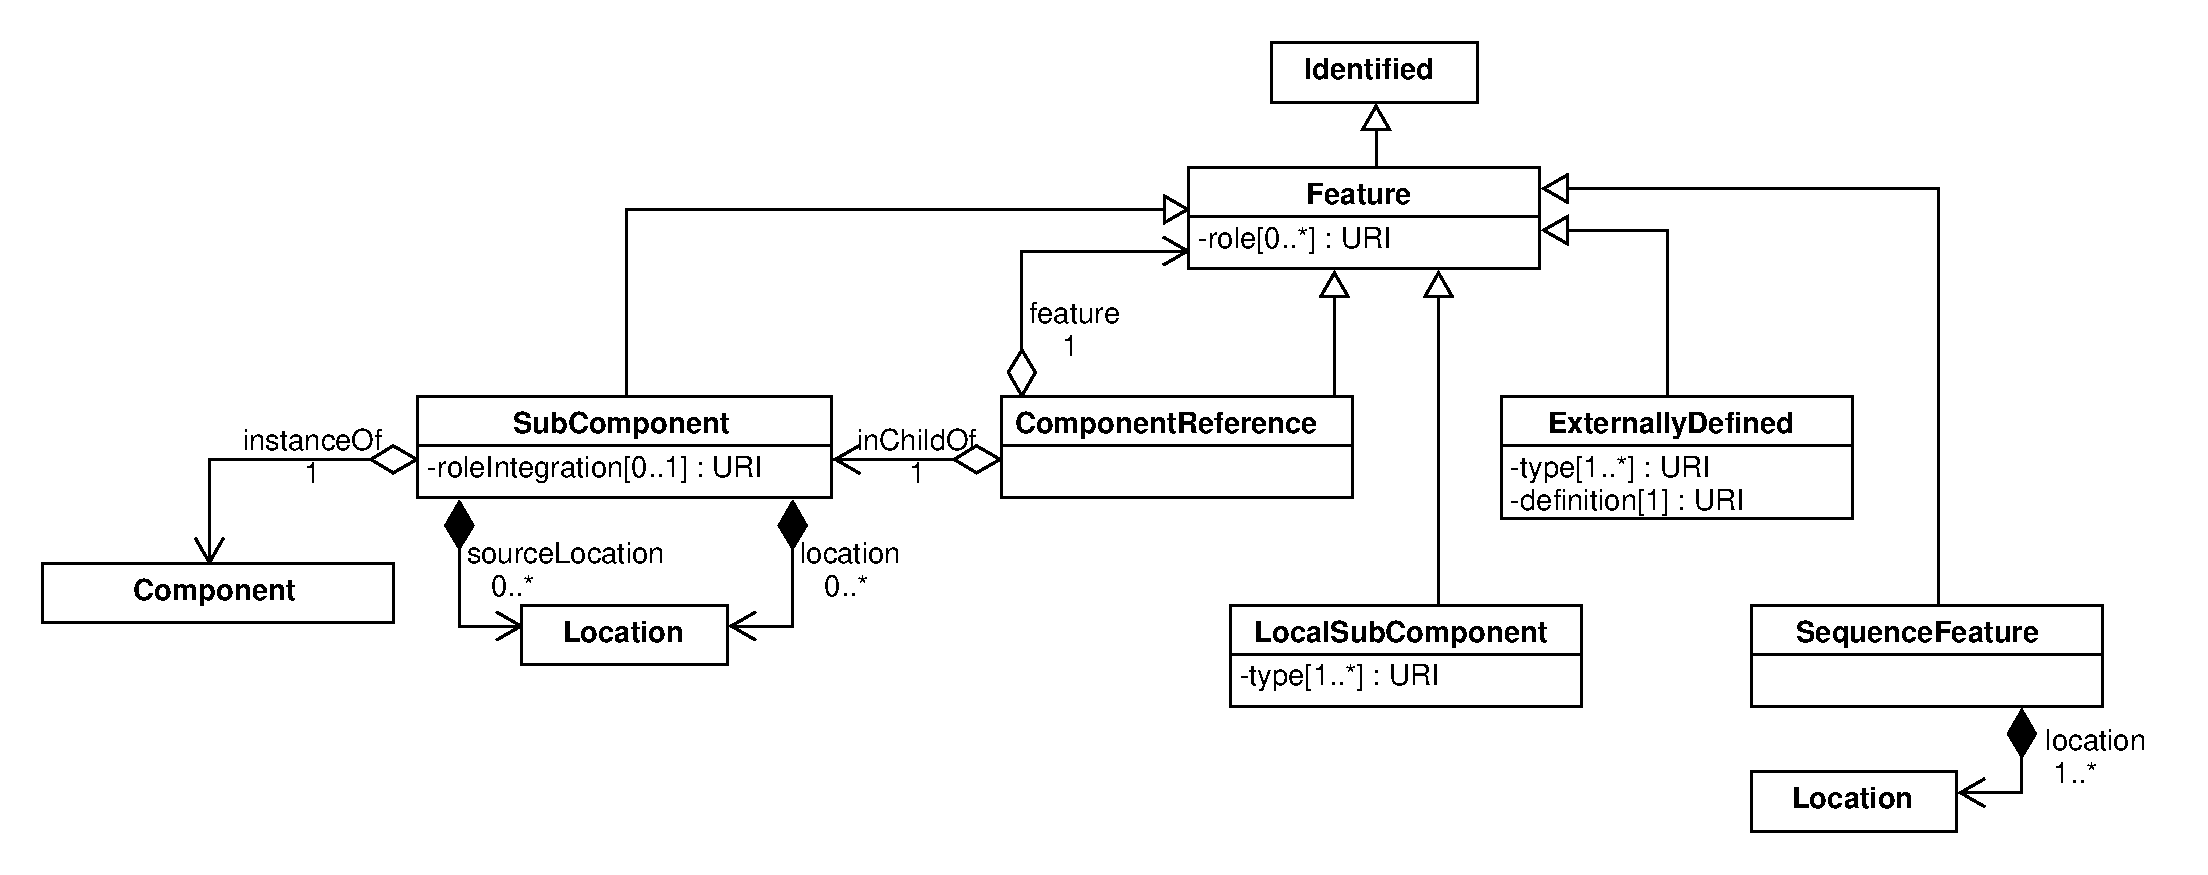
\includegraphics[width=\textwidth]{uml/feature}
\caption[]{Diagram of the \sbol{Feature} class and its associated properties.}
\label{uml:subcomponent}
\end{center}
\end{figure}

The \sbol{Feature} class is used to compose \sbol{Component} objects into a structural or functional hierarchy. 

\subparagraph{The \sbolheading{role} property}\label{sec:roles:C}

The expected purpose and function of a genetic part are described by the
\sbolmult{roles:CD}{roles} property of \sbol{Component}. However, the same building block might be used for a different purpose in an actual design. In other words, purpose and function are sometimes determined by context. 

The \sbolmult{roles:C}{roles} property comprises an OPTIONAL set of zero or more \sbolmult{roles:C}{role} \sbol{URI}s describing the purpose or potential function of this \sbol{Feature}'s included sub-\sbol{Component} in the \textit{context} of its parent \sbol{Component}.
If provided, these \sbolmult{roles:C}{role} \sbol{URI}s MUST identify terms from appropriate ontologies. Roles are not restricted to describing biological function; they may annotate a \sbol{Feature}'s function in any domain for which an ontology exists.

It is RECOMMENDED that these \sbolmult{roles:C}{role} \sbol{URI}s identify terms that are compatible with the \sbolmult{types:CD}{type} properties of both this \sbol{Feature}'s parent \sbol{Component} and its included sub-\sbol{Component}. For example, a \sbolmult{roles:C}{role} of a \sbol{Feature} which belongs to a \sbol{Component} of type DNA and includes a sub-\sbol{Component} of type DNA might refer to terms from the Sequence Ontology. A table of recommended ontology terms for \sbolmult{roles:C}{roles} is given in \ref{tbl:component_roles}.

\paragraph{SubComponent}
\label{sec:SubComponent}

The \sbol{SubComponent} class a subclass of the \sbol{Feature} class that can be used to specify structural hierarchy. For example, the \sbol{Component} of a gene could contain four \sbol{SubComponent} objects: a promoter, RBS, CDS, and terminator. In turn, the \sbol{Component} of the promoter \sbol{SubComponent} could contain \sbol{SubComponent} objects defined as various operator sites.

\subparagraph{The \sbolheading{roleIntegration} property}\label{sec:roleIntegration:C}


A \sbolmult{roleIntegration:C}{roleIntegration} specifies the relationship between a \sbol{Feature} instance's own set of \sbolmult{roles:C}{roles} and the set of \sbolmult{roles:CD}{roles} on the included sub-\sbol{Component}.

The \sbolmult{roleIntegration:C}{roleIntegration} property has a data type of \sbol{URI}. A \sbol{Feature} instance with zero \sbolmult{roles:C}{roles} MAY OPTIONALLY specify a \sbolmult{roleIntegration:C}{roleIntegration}. A \sbol{Feature} instance with one or more \sbolmult{roles:C}{roles} MUST specify a \sbolmult{roleIntegration:C}{roleIntegration} from \ref{tbl:component_roleIntegration}.
If zero \sbol{Feature} \sbolmult{roles:C}{roles} are given and no \sbol{Feature} \sbolmult{roleIntegration:C}{roleIntegration} is given, then \url{http://sbols.org/v2\#mergeRoles} is assumed.
It is RECOMMENDED to specify a set of \sbol{Feature} \sbolmult{roles:C}{roles} only if the integrated result set of roles would differ from the set of \sbolmult{roles:CD}{roles} belonging to this \sbol{Feature}'s included sub-\sbol{Component}.


\begin{table}[ht]
  \begin{edtable}{tabular}{lp{4in}}
    \toprule
    \textbf{roleIntegration URI} & \textbf{Description} \\
    \midrule
    \url{http://sbols.org/v2\#overrideRoles} & In the context of this \sbol{Feature}, ignore any \sbolmult{roles:CD}{roles} given for the included sub-\sbol{Component}. Instead use only the set of zero or more \sbolmult{roles:C}{roles} given for this \sbol{Feature}. \\
    \url{http://sbols.org/v2\#mergeRoles} & Use the union of the two sets: both the set of zero or more \sbolmult{roles:C}{roles} given for this \sbol{Feature} as well as the set of zero or more \sbolmult{roles:CD}{roles} given for the included sub-\sbol{Component}. \\
    \bottomrule
  \end{edtable}
  \caption{Each \sbolmult{roleIntegration:C}{roleIntegration} mode is associated with a rule governing how a \sbol{Feature}'s roles are to be combined with the included 
sub-\sbol{Component}'s roles.}
  \label{tbl:component_roleIntegration}
\end{table}


\subparagraph{The \sbolheading{instanceOf} property}
\label{sec:instanceOf}

The \sbol{instanceOf} property is a REQUIRED \sbol{URI} that refers to the \sbol{Component} of the \sbol{Feature}.
As described in the previous section, this \sbol{Component} effectively provides information about the \sbolmult{types:CD}{types} and \sbolmult{roles:CD}{roles} of the \sbol{Feature}.

The \sbol{instanceOf} property MUST NOT refer to the same \sbol{Component} as the one that contains the \sbol{Feature}.
Furthermore, \sbol{Feature} objects MUST NOT form a cyclical chain of references via their \sbol{instanceOf} properties and the \sbol{Component} objects that contain them.
For example, consider the \sbol{Feature} objects $A$ and $B$ and the \sbol{Component} objects $X$ and $Y$. The reference chain ``$X$ contains $A$, $A$ is defined by $Y$, $Y$ contains $B$, and $B$ is defined by $X$'' is cyclical.

The \sbol{sourceLocations} property is an OPTIONAL set of zero or more \sbol{Location} objects that indicate which \sbol{elements} of a \sbol{Component}'s \sbol{Sequence} are to be included in the \sbol{Component}'s parent. The \sbol{sourceLocations} property
allows for only a portion of a \sbol{Component}'s \sbol{Sequence} to be included, rather than its entirety.

If the \sbol{sourceLocation} property is not set, then the whole \sbol{Sequence} is assumed to be included. Alternatively,
if the \sbol{sourceLocation} property is set, then the relationship between the original \sbol{Component}'s
\sbol{Sequence} and the included \sbol{Sequence} is defined identically to the \sbol{locations}
property on the \sbol{SequenceFeature} object.


\subparagraph{The \sbolheading{location} property}\label{sec:location}
The \sbol{location} property is an OPTIONAL set which points to a \sbol{Location} on the parent \sbol{Component} sequence; if \sbol{location} is missing, this indicates a part / sub-part relationship for which sequence details have not (yet) been determined.

The \sbol{Location} record(s) specified by a \sbol{Feature} are subject to the same restrictions currently in place for \sbol{SequenceFeature} \sbol{Location}. Concretely, two \sbol{Location} records attached to the same \sbol{Feature} MUST NOT overlap in their range as it would not be clear what that means. The \sbol{Location} of two separate \sbol{Feature}s may overlap.

\subparagraph{The \sbolheading{orientation} property}\label{sec:orientation2}
The \sbol{orientation} property is OPTIONAL and has a data type of \sbol{URI}. All subclasses of \sbol{Feature} share this property, which can be used to indicate how the region specified by the \sbol{SequenceFeature} and any associated double-stranded \sbol{SubComponent} is oriented on the \sbol{elements} of a \sbol{Sequence}  from their parent \sbol{Component}. \ref{tbl:orientation_types} provides a list of REQUIRED \sbol{orientation} \sbol{URI}s. If a \sbol{Feature} object has an \sbol{orientation}, then it MUST come from \ref{tbl:orientation_types}.

\todo{add best practice here talking about EntireComponent?}


\paragraph{ComponentReference}
\label{sec:ComponentReference}

The \sbol{ComponentReference} class is a subclass of \sbol{Feature} and a sibling of the \sbol{SubComponent} class. 


\subparagraph{The \sbolheading{inChildOf} property}\label{sec:inChildOf}

The \sbol{inChildOf} property is a REQUIRED \sbol{URI} that refers to a SubComponent. \sbol{inChildOf} must refer to a \sbol{SubComponent} pointed directly to by the parent of the \sbol{ComponentReference} (i.e., as a \sbol{SubComponent} of \sbol{Component}, or an \sbol{inChildOf} of \sbol{ComponentReference}). If the \sbol{Feature} is a \sbol{SubComponent}, then it must be a child of the \sbol{SubComponent} pointed to by \sbol{inChildOf}.

\subparagraph{The \sbolheading{feature} property}\label{sec:feature:CR}

The \sbolmult{feature:CR}{feature} property is an OPTIONAL \sbol{URI} that refers to a \sbol{Feature}.

\paragraph{LocalSubComponent}
\label{sec:LocalSubComponent}

The \sbol{LocalSubComponent} class a subclass of \sbol{Feature}. This class was serves as a way to create an ``empty'' \sbol{Component} to serve as a placeholder in more complex \sbol{Component}s. 

\subparagraph{The \sbolheading{type} property}\label{sec:type:LSC}

The \sbolmult{type:LSC}{type} property is REQUIRED and contains one or more \sbol{URI}s. The \sbolmult{type:LSC}{type} property is identical to its use in \sbol{Component}

\paragraph{ExternallyDefined}
\label{sec:ExternallyDefined}

The \sbol{ExternallyDefined} class has been introduced so that external definitions in databases like CHEBI or UniProt can be referenced.

\subparagraph{The \sbolheading{type} property}\label{sec:type:ED}

The \sbolmult{type:ED}{type} property is REQUIRED and contains one or more \sbol{URI}s. The \sbolmult{type:ED}{type} property is identical to its use in \sbol{Component}

\subparagraph{The \sbolheading{definition} property}\label{sec:definition:ER}

The \sbolmult{definition:ER}{definition} property is REQUIRED and contains one \sbol{URI} that links to a cononical definition external to SBOL.


\paragraph{SequenceFeature}
\label{sec:SequenceFeature}

The \sbol{SequenceFeature} class describes one or more regions of interest on the \sbol{Sequence} objects referred to by its parent \sbol{Component}. 
%In addition, \sbol{SequenceFeature} objects can describe the substructure of their parent \sbol{Component} through association with the \sbol{Feature} objects contained by this \sbol{Component}.

\subparagraph{The \sbolheading{locations} property}\label{sec:locations}
The \sbol{locations} property is a REQUIRED set of one or more \sbol{Location} objects that indicate which \sbol{elements} of a \sbol{Sequence} are described by the \sbol{SequenceFeature}.

Allowing multiple \sbol{Location} objects on a single \sbol{SequenceFeature} is intended to enable representation of discontinuous regions (for example, a \sbol{Feature} encoded across a set of exons with interspersed introns).
As such, the \sbol{Location} objects of a single \sbol{SequenceFeature} SHOULD NOT specify overlapping regions, since it is not clear what this would mean.
There is no such concern with different \sbol{SequenceFeature} objects, however, which can freely overlap in \sbol{Location} (for example, specifying overlapping linkers for sequence assembly).

\subsubsection{Location}
\label{sec:Location}
The \sbol{Location} class is extended by the \sbol{Range}, \sbol{Cut}, and \sbol{EntireSequence} classes.

\begin{figure}[ht]
\begin{center}
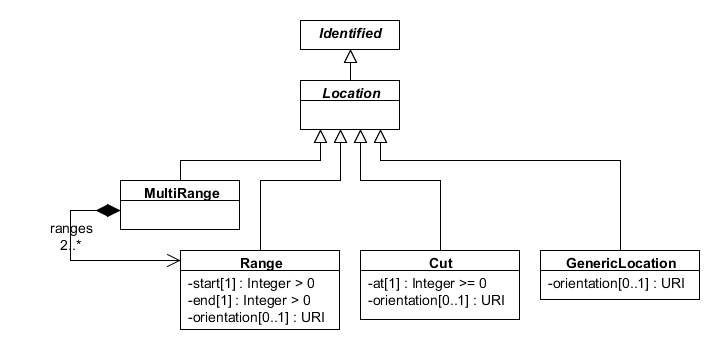
\includegraphics[scale=0.6]{uml/location}
\caption[]{Diagram of the \sbol{Location} class and its associated properties.}
\label{uml:location}
\end{center}
\end{figure} \todo{change diagram to reflect changes from SEP 41}

\subparagraph{The \sbolheading{orientation} property}
\label{sec:orientation}
The \sbol{orientation} property is OPTIONAL and has a data type of \sbol{URI}. All subclasses of \sbol{Location} share this property, which can be used to indicate how the region specified by the \sbol{SequenceFeature} and any associated double-stranded \sbol{Feature} is oriented on the \sbol{elements} of a \sbol{Sequence}  from their parent \sbol{Component}. \ref{tbl:orientation_types} provides a list of REQUIRED \sbol{orientation} \sbol{URI}s. If a \sbol{Location} object has an \sbol{orientation}, then it MUST come from \ref{tbl:orientation_types}.

\subparagraph{The \sbolheading{sequence} property}
\label{sec:sequence}
The \sbol{sequence} property is REQUIRED and MUST contain the \sbol{URI} of a \sbol{Sequence} object. All subclasses of \sbol{Location} share this property, which indicates which \sbol{Sequence} object referenced by the containing \sbol{Component} is referenced by the \sbol{Location}.

\begin{table}[ht]
  \begin{edtable}{tabular}{lp{3.75in}}
    \toprule
    \textbf{Orientation URI} & \textbf{Description} \\
    \midrule
    \url{http://sbols.org/v2\#inline} & The region specified by this \sbol{Location} is on the \sbol{elements} of a \sbol{Sequence}. \\
    \url{http://sbols.org/v2\#reverseComplement} & The region specified by this \sbol{Location} is on the reverse-complement translation of the \sbol{elements} of a \sbol{Sequence}. The exact nature of this translation depends on the \sbol{encoding} of the \sbol{Sequence}. \\
    \bottomrule
  \end{edtable}
  \caption{REQUIRED \sbol{URI}s for the \sbol{orientation} property}
  \label{tbl:orientation_types}
\end{table}


\paragraph{Range}
\label{sec:Range}
A \sbol{Range} object specifies a region via discrete, inclusive \sbol{start} and \sbol{end} positions that correspond to indices for characters in the \sbol{elements} \sbol{String} of a \sbol{Sequence}.

Note that the index of the first location is 1, as is typical practice in biology, rather than 0, as is typical practice in computer science.

\subparagraph{The \sbolheading{start} property}\label{sec:start}
The \sbol{start} property specifies the inclusive starting position of the \sbol{Range}. This property is REQUIRED and MUST contain an \sbol{Integer} value greater than zero.

\subparagraph{The \sbolheading{end} property}\label{sec:end}
The \sbol{end} property specifies the inclusive ending position of the \sbol{Range}. This property is REQUIRED and MUST contain an \sbol{Integer} value greater than zero. In addition, this \sbol{Integer} value MUST be greater than or equal to that of the \sbol{start} property.

\paragraph{Cut}
\label{sec:Cut}
The \sbol{Cut} class has been introduced to enable the specification of a region between two discrete positions.
This specification is accomplished using the \sbol{at} property, which specifies a discrete position that that corresponds to the index of a character in the \sbol{elements} \sbol{String} of a \sbol{Sequence} (except in the case when \sbol{at} is equal to zero---see below).

\subparagraph{The \sbolheading{at} property}
\label{sec:at}
The \sbol{at} property is REQUIRED and MUST contain an \sbol{Integer} value greater than or equal to zero. The region specified by the \sbol{Cut} is between the position specified by this property and the position that immediately follows it. When the \sbol{at} property is equal to zero, the specified region is immediately before the first discrete position or character in the \sbol{elements} \sbol{String} of a \sbol{Sequence}.


\paragraph{EntireSequence}
\label{sec:EntireSequence}
The \sbol{EntireSequence} class does not have any additional properties. Use of this class indicates that the linked Sequence describes the entirety of the \sbol{Component} or \sbol{Feature} parent of this Location object.

\subparagraph{The \sbolheading{order} property}
\label{sec:order}


\subsubsection{Constraint}
\label{sec:Constraint}
The \sbol{Constraint} class can be used to assert restrictions on the relationships of pairs of \sbol{Feature} objects contained by the same parent \sbol{Component}.
Uses of this class include expressing containment (e.g., a plasmid transformed into a chassis strain), identity mappings (e.g., replacing a placeholder value with a complete definition), and expressing relative, sequence-based positions (e.g., the ordering of features within a template).
Each \sbol{Constraint} includes the \sbol{restriction}, \sbol{subject}, and \sbol{object} properties.

\begin{figure}[ht]
\begin{center}
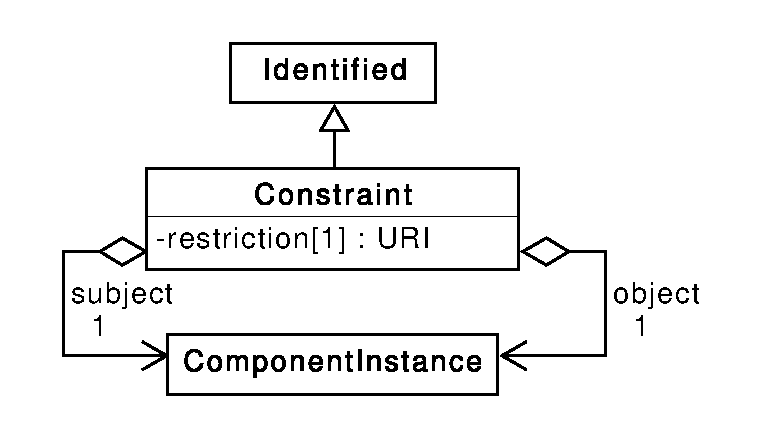
\includegraphics[scale=0.6]{uml/constraint}
\caption[]{Diagram of the \sbol{Constraint} class and its associated properties.}
\label{uml:sequence_constraint}
\end{center}
\end{figure}

\subparagraph{The \sbolheading{subject} property}\label{sec:subject}
The \sbol{subject} property is REQUIRED and MUST contain a \sbol{URI} that refers to a \sbol{Feature} contained by the same parent \sbol{Component} that contains the \sbol{Constraint}.

\subparagraph{The \sbolheading{object} property}\label{sec:object}
The \sbol{object} property is REQUIRED and MUST contain a \sbol{URI} that refers to a \sbol{Feature} contained by the same parent \sbol{Component} that contains the \sbol{Constraint}. This \sbol{Feature} MUST NOT be the same \sbol{Feature} that the \sbol{Constraint} refers to via its \sbol{subject} property.

\subparagraph{The \sbolheading{restriction} property}\label{sec:restriction}

The \sbol{restriction} property is REQUIRED and has a data type of \sbol{URI}. 
This property MUST indicate the type of restriction on the locations, orientations, or identities of the \sbol{subject} and \sbol{object} \sbol{ComponentInstance} objects in relation to each other. 
The \sbol{URI} value of this property SHOULD come from the RECOMMENDED \sbol{URI}s in \ref{tbl:restriction_types_identity}, \ref{tbl:restriction_types_topology}, and \ref{tbl:restriction_types_sequence}.

% identify and orientation
\begin{table}[ht]
  \begin{edtable}{tabular}{lp{3.25in}}
    \toprule
    \textbf{Restriction URI} & \textbf{Description} \\
    \midrule
    % identity relations
	\url{http://sbols.org/v3#verifyIdentical}  & The \sbol{instanceOf} properties of the \sbol{subject} and \sbol{object} \sbol{Feature} objects MUST refer to the same \sbol{Component}.  \emph{Example: a promoter included via two different subsystems must be the identical.} \\
	\url{http://sbols.org/v3\#differentFrom} & The \sbol{instanceOf} property of the \sbol{subject} \sbol{Feature} MUST NOT refer to the same \sbol{Component} as that of the \sbol{object} \sbol{Component}. \emph{Example: two fluorescent reporters must be different.}\\
	\url{http://sbols.org/v3#replaces} &	In the context of the parent object of the \sbol{Constraint}, information about the \sbol{subject} should be used in place of all instances of the \sbol{object}. \emph{Example: the J23101 promoter replaces a generic promoter.} \\
    
    % orientation relations
	\url{http://sbols.org/v3\#sameOrientationAs} & The \sbol{subject} and \sbol{object} \sbol{Component} objects MUST have the same orientation. \emph{Example: a promoter has the same orientation as the coding sequence it controls.}\\
	\url{http://sbols.org/v2\#oppositeOrientationAs} & The \sbol{subject} and \sbol{object} \sbol{Component} objects MUST have opposite orientations. \emph{Example: a promoter has the opposite orientation as an invertase-activated coding sequence it controls.}\\

    \bottomrule
  \end{edtable}
  \caption{RECOMMENDED \sbol{URI}s for expressing identity and orientation with the \sbol{restriction} property.}
  \label{tbl:restriction_types_identity}
\end{table}

    % topology relations
\begin{table}[ht]
  \begin{edtable}{tabular}{lp{3.25in}}
    \toprule
    \textbf{Restriction URI} & \textbf{Description} \\
    \midrule
	\url{http://sbols.org/v3#isDisjointFrom}	& The \sbol{subject} and \sbol{object} do not overlap in space. \emph{Example: a plasmid is disjoint from a chromosome.} \\
	\url{http://sbols.org/v3#strictlyContains} &	The \sbol{subject} entirely contains the \sbol{object}: they do not share a boundary. \emph{Example: a cell contains a plasmid} \\
	\url{http://sbols.org/v3#contains} &	The \sbol{subject} contains the \sbol{object} and they might or might not share a boundary (i.e., union of {\tt strictlyContains}, {\tt equals}, and {\tt covers}. \emph{Example: a cell contains a protein that may or may not bind to its membrane.} \\
	\url{http://sbols.org/v3#equals} &	The \sbol{subject} and \sbol{object} occupy the same location in space. \emph{Example: a small molecule is distributed throughour an entire sample.} \\
	\url{http://sbols.org/v3#meets} &	The \sbol{subject} and \sbol{object} are connected at a shared boundary. \emph{Example: two strains of adherent cells meet at their membranes.} \\
	\url{http://sbols.org/v3#covers} &	The \sbol{subject} contains the \sbol{object} but also shares a boundary. \emph{Example: a cell covers its transmembrane proteins.} \\
	\url{http://sbols.org/v3#overlaps} &	The \sbol{subject} and \sbol{object} overlap in space, but portions of each are outside of the other. \emph{Example: a transmembrane protein overlaps the cell membrane.} \\
    \bottomrule
  \end{edtable}
  \caption{RECOMMENDED \sbol{URI}s for expressing topological relations with the \sbol{restriction} property.}
  \label{tbl:restriction_types_topology}
\end{table}

\begin{table}[ht]
  \begin{edtable}{tabular}{lp{3.25in}}
    \toprule
    \textbf{Restriction URI} & \textbf{Description} \\
    \midrule
    % linear relations
	\url{http://sbols.org/v3#precedes} &	The start of the location for \sbol{subject} is less than the start of the location for \sbol{object} (i.e., union of \sbol{strictlyPrecedes}, \sbol{meets}, and \sbol{overlaps}). 
	\emph{Example: a promoter precedes a ribosome entry site, but the exact boundary between the two will be determined by sequence optimization and assembly planning}. \\
	
	\url{http://sbols.org/v3#strictlyPrecedes} &	The end of the location for \sbol{subject} is less than the start of the location for \sbol{object}. 
	\emph{Example: a promoter strictly precedes a terminator (with a CDS between them).} \\
	
	\url{http://sbols.org/v3#meets} &	The end of the location for \sbol{subject} is equal to the start of the location for \sbol{object}. 
	Note: this is a stronger interpretation of {\tt meets} from \ref{tbl:restriction_types_topology} in the context of a linear sequence.
	\emph{Example: the 3' region adjacent to a blunt restriction site meets the 5' region adjacent to the site.} \\
	
	\url{http://sbols.org/v3#overlaps} &	The start of the location for \sbol{subject} is before the start of the location for \sbol{object} and the end of the location for \sbol{subject} is before the end of the location for \sbol{object}. 
	Note: this is a stronger interpretation of {\tt overlaps} from \ref{tbl:restriction_types_topology} in the context of a linear sequence.
	\emph{Example: two oligos in a Gibson assembly plan} \\
	
	\url{http://sbols.org/v3#contains} &	The start of the location for \sbol{subject} is less than or equal to the start of the location for \sbol{object} and the end of the location for \sbol{subject} is greater than or equal to the end of the location for \sbol{object} (i.e., union of {\tt strictlyContains}, {\tt equals}, {\tt finishes}, and {\tt starts}). 
	Note: this is a stronger interpretation of {\tt contains} from \ref{tbl:restriction_types_topology} in the context of a linear sequence.
	\emph{Example: a composite part contains a promoter} \\
	
	\url{http://sbols.org/v3#strictlyContains} &	The start of the location for \sbol{subject} is before the start of the location for \sbol{object} and the end of the location for \sbol{subject} is after the end of the location for \sbol{object}. 
	Note: this is a stronger interpretation of {\tt strictlyContains} from \ref{tbl:restriction_types_topology} in the context of a linear sequence.
	\emph{Example: an RNA transcript strictly contains an intron.} \\
	
	\url{http://sbols.org/v3#equals} &	The start and end of the location for \sbol{subject} are equal to the start and end of the location for \sbol{object}. 
	Note: this is a stronger interpretation of {\tt equals} from \ref{tbl:restriction_types_topology} in the context of a linear sequence.
	\emph{Example: the transcribed region of a CDS part equals the entire part.} \\
	
	\url{http://sbols.org/v3#finishes} &	The start of the location for \sbol{subject} is after the start of the location for \sbol{object} and the end of the location for \sbol{subject} is equal to the end of the location for \sbol{object}. 
	\emph{Example: a terminator finishes an expression cassette.} \\
	
	\url{http://sbols.org/v3#starts} &	The start of the location for \sbol{subject} is equal to the start of the location for \sbol{object} and the end of the location for \sbol{subject} is before the end of the location for \sbol{object}. 
	\emph{Example: a promoter starts an expression cassette.} \\
    \bottomrule
  \end{edtable}
  \caption{RECOMMENDED \sbol{URI}s for expressing sequential relations with the \sbol{restriction} property.}
  \label{tbl:restriction_types_sequence}
\end{table}


\subsubsection{Interaction}
\label{sec:Interaction}

\begin{figure}[ht]
\begin{center}
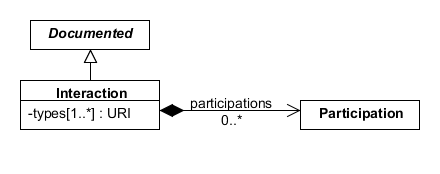
\includegraphics[scale=0.6]{uml/interaction}
\caption[]{Diagram of the \sbol{Interaction} class and its associated properties.}
\label{uml:interaction}
\end{center}
\end{figure}

The \sbol{Interaction} class provides more detailed description of how the \sbol{Feature} objects of a\\ \sbol{Component} are intended to work together.
For example, this class can be used to represent different forms of genetic regulation (e.g., transcriptional activation or repression), processes from the central dogma of biology (e.g. transcription and translation), and other basic molecular interactions (e.g., non-covalent binding or enzymatic phosphorylation).
Each \sbol{Interaction} includes a \sbolmult{types:I}{types} property that refers to descriptive ontology terms and a \sbol{participations} property that describes which \sbol{Feature} objects participate in the \sbol{Interaction}.

\subparagraph{The \sbolheading{types} property}\label{sec:types:I}

The \sbolmult{types:I}{types} property is a REQUIRED set of \sbol{URI}s that describes the behavior represented by an \sbol{Interaction}.

The \sbolmult{types:I}{types} property MUST contain one or more \sbol{URI}s that MUST identify terms from appropriate ontologies. It is RECOMMENDED that exactly one \sbol{URI} contained by the \sbolmult{types:I}{types} property refer to a term from the occurring entity branch of the Systems Biology Ontology (SBO). (See \url{http://www.ebi.ac.uk/sbo/main/}) \ref{tbl:interaction_types} provides a list of possible SBO terms for the \sbolmult{types:I}{types} property and their corresponding \sbol{URI}s.

\begin{table}[ht]
  \begin{edtable}{tabular}{ll}
    \toprule
    \textbf{Interaction Type} & \textbf{URI for SBO Term} \\
    \midrule
    Inhibition  & \url{http://identifiers.org/biomodels.sbo/SBO:0000169}\\
    Stimulation & \url{http://identifiers.org/biomodels.sbo/SBO:0000170}\\
    Biochemical Reaction & \url{http://identifiers.org/biomodels.sbo/SBO:0000176}\\
    Non-Covalent Binding & \url{http://identifiers.org/biomodels.sbo/SBO:0000177}\\
    Degradation & \url{http://identifiers.org/biomodels.sbo/SBO:0000179}\\
    Genetic Production & \url{http://identifiers.org/biomodels.sbo/SBO:0000589}\\
    Control  & \url{http://identifiers.org/biomodels.sbo/SBO:0000168} \\
    \bottomrule
  \end{edtable}
  \caption{SBO terms to specify the \sbolmult{types:I}{types} property of an \sbol{Interaction}.}
  \label{tbl:interaction_types}
\end{table}

If an \sbol{Interaction} is well described by one of the terms from \ref{tbl:interaction_types}, then its \sbolmult{types:I}{types} property MUST contain the \sbol{URI} that identifies this term. Lastly, if the \sbolmult{types:I}{types} property of an \sbol{Interaction} contains multiple
 \sbol{URI}s, then they MUST identify non-conflicting terms. For example, the SBO terms ``stimulation'' and ``inhibition'' would conflict.

\subparagraph{The \sbolheading{participations} property}\label{sec:participations}

The \sbol{participations} property is an OPTIONAL and MAY contain a set of \sbol{Participation} objects, each of which identifies the \sbolmult{roles:P}{roles} that its referenced \sbol{Feature} plays in the \sbol{Interaction}.

Even though an \sbol{Interaction} generally contains at least one \sbol{Participation}, the case of zero \sbol{Participation} objects is allowed because it is plausible that a designer might want to specify that an \sbol{Interaction} will exist, even if its \sbol{participant}s have not yet been determined.

\begin{figure}[ht]
\begin{center}
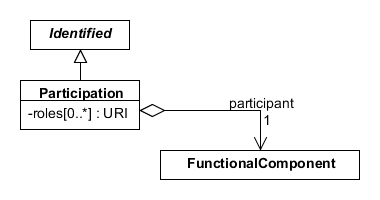
\includegraphics[scale=0.6]{uml/participation}
\caption[]{Diagram of the \sbol{Participation} class and its associated properties.}
\label{uml:participation}
\end{center}
\end{figure}

\subsubsection{Participation}
\label{sec:Participation}

Each \sbol{Participation} represents how a particular \sbol{Feature} behaves in its parent
\sbol{Interaction}.

\subparagraph{The \sbolheading{roles} property}\label{sec:roles:P}

The \sbolmult{roles:P}{roles} property is a REQUIRED set of \sbol{URI}s that describes the behavior of a \sbol{Participation} (and by extension its referenced \sbol{Feature}) in the context of its parent \sbol{Interaction}.

The \sbolmult{roles:P}{roles} property MUST contain one or more \sbol{URI}s that MUST identify terms from appropriate ontologies. It is RECOMMENDED that exactly one \sbol{URI} contained by the \sbolmult{roles:P}{roles} property refer to a term from the participant role branch of the SBO. \ref{tbl:participant_roles} provides a list of possible SBO terms for the \sbolmult{roles:P}{roles} property and their corresponding \sbol{URI}s.

\begin{table}[ht]
  \begin{edtable}{tabular}{lll}
    \toprule
    \textbf{Participation Role} & \textbf{URI for SBO Term} & \textbf{Interaction Types}\\
    \midrule
    Inhibitor  & \url{http://identifiers.org/biomodels.sbo/SBO:0000020} & Inhibition\\
    Inhibited  & \url{http://identifiers.org/biomodels.sbo/SBO:0000642} & Inhibition\\
    Stimulator & \url{http://identifiers.org/biomodels.sbo/SBO:0000459}  & Stimulation\\
    Stimulated & \url{http://identifiers.org/biomodels.sbo/SBO:0000643}  & Stimulation\\
     Reactant & \url{http://identifiers.org/biomodels.sbo/SBO:0000010}  & Non-Covalent Binding, Degradation \\
     & & Biochemical Reaction \\
    Product & \url{http://identifiers.org/biomodels.sbo/SBO:0000011}  & Non-Covalent Binding, \\
    & & Genetic Production, Biochemical Reaction\\
    Promoter  & \url{http://identifiers.org/biomodels.sbo/SBO:0000598} & Inhibition, Stimulation, Genetic Production\\
    Modifier  & \url{http://identifiers.org/biomodels.sbo/SBO:0000019} & Biochemical Reaction, Control\\
    Modified  & \url{http://identifiers.org/biomodels.sbo/SBO:0000644} & Biochemical Reaction, Control\\
    Template  & \url{http://identifiers.org/biomodels.sbo/SBO:0000645} & Genetic Production\\
%    Ligand & \url{http://identifiers.org/biomodels.sbo/SBO:0000280}\\
%    Non-Covalent Complex & \url{http://identifiers.org/biomodels.sbo/SBO:0000253}\\
    \bottomrule
  \end{edtable}
  \caption{SBO terms to specify the \sbolmult{roles:P}{roles} property of a \sbol{Participation}.}
  \label{tbl:participant_roles}
\end{table}

If a \sbol{Participation} is well described by one of the terms from \ref{tbl:participant_roles}, then its \sbolmult{roles:P}{roles} property MUST contain the \sbol{URI} that identifies this term.
Also, if a \sbol{Participation} belongs to an \sbol{Interaction} that has a type listed in \ref{tbl:interaction_types}, then the \sbol{Participation} SHOULD have a role that is cross-listed with this type in \ref{tbl:participant_roles}.
Lastly, if the \sbolmult{roles:P}{roles} property of a \sbol{Participation} contains multiple
 \sbol{URI}s, then they MUST identify non-conflicting terms. For example, the SBO terms ``stimulator'' and ``inhibitor'' would conflict.


\subparagraph{The \sbolheading{participant} property}\label{sec:participant}

The \sbol{participant} property MUST specify precisely one \sbol{Feature} object that plays the designated role in its parent \sbol{Interaction} object.


\subsubsection{Interface}
\label{sec:Interface}

\begin{figure}[ht]
\begin{center}
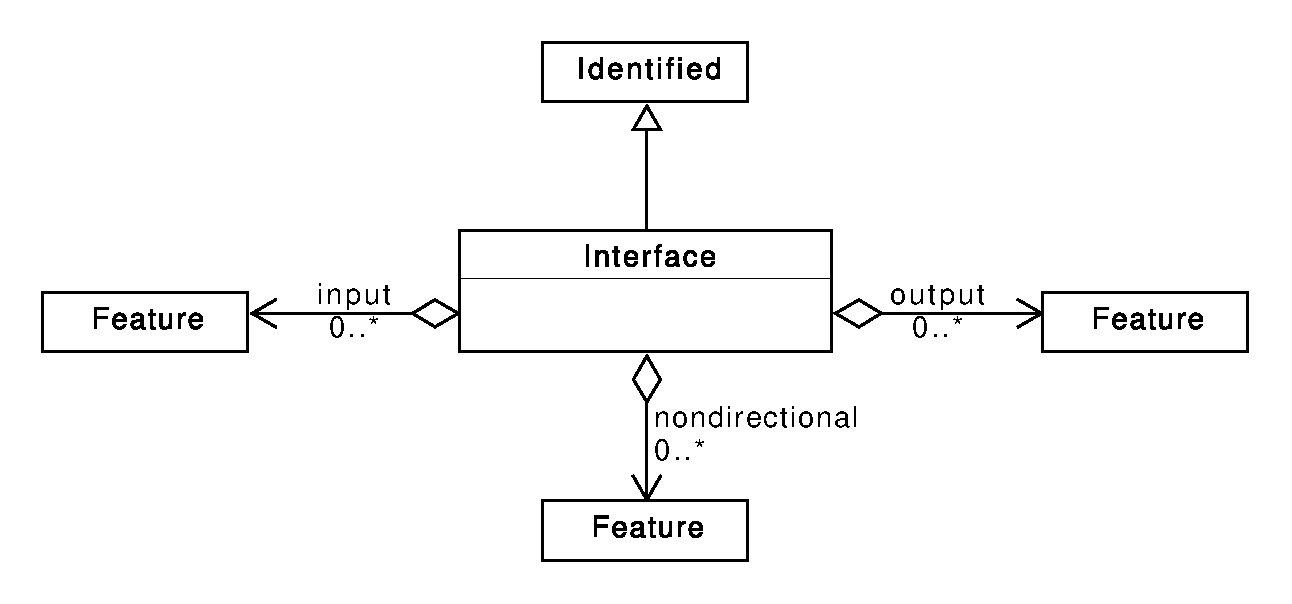
\includegraphics[scale=0.6]{uml/interface}
\caption[]{Diagram of the \sbol{Interface} class and its associated properties.}
\label{uml:interface}
\end{center}
\end{figure}

The \sbol{Interface} class is a way of explicitly specifying the interface of a \sbol{Component}. 

\subparagraph{The \sbolheading{input} property}
\label{sec:input:Interface}
The \sbolmult{input:Interface}{input} property is OPTIONAL and MAY contain a set of \sbol{Feature} \sbol{URI}s in the same \sbol{Component}.
\subparagraph{The \sbolheading{output} property}
\label{sec:output:Interface}
The \sbolmult{output:Interface}{output} property is OPTIONAL and MAY contain a set of \sbol{Feature} \sbol{URI}s in the same \sbol{Component}.

\subparagraph{The \sbolheading{nondirectional} property}
\label{sec:nondirectional:Interface}
The \sbolmult{nondirectional:Interface}{nondirectional} property is OPTIONAL and MAY contain a set of \sbol{Feature} \sbol{URI}s in the same \sbol{Component}. Note that nondirectional can imply both bidirectional as well as situations where there are no flows (for instance - a physical interface).



